% questions.tex —— 2014 年·北京卷·理科 · 题目内容片段（无答案）
% 由 tools/generate_projects.py 依来源总账自 2014/2014_数学真题_北京理_试题.md 生成，勿手改（改源 MD 后重跑）


\begin{gknotice}
\textbf{来源说明}：本题面依据固定源 PDF 的两页 A3 题面逐题转录，原卷印刷页码为 861—862。第 861 面为选择题 1—8、填空题 9—14，以及解答题 15—17 的题干；第 862 面为解答题 18—20。全卷不印分值，三处节头依次为「一、选择题」「二、填空题」「三、解答题」。

\textbf{图形说明}：第 4 题程序框图、第 15 题三角形、第 17 题五棱锥，均由项目内 TikZ 矢量源重绘；其余各题原页无图。

\textbf{解析归属}：固定源不附答案或解析；配套答案与解析均由本库按本题面独立复算。
\end{gknotice}

\gkpart{一、选择题}

\begin{question}
\gkti{1}已知集合 $A=\{x\mid x^2-2x=0\}$，$B=\{0,1,2\}$，则 $A\cap B=$\mbox{（　　）}

（A）$\{0\}$；（B）$\{0,1\}$；（C）$\{0,2\}$；（D）$\{0,1,2\}$。

\end{question}
\begin{question}
\gkti{2}下列函数中，在区间 $(0,+\infty)$ 上为增函数的是\mbox{（　　）}

（A）$y=\sqrt{x+1}$；（B）$y=(x-1)^2$；（C）$y=2^{-x}$；（D）$y=\log_{0.5}(x+1)$。

\end{question}
\begin{question}
\gkti{3}曲线
\nopagebreak[4]
\[\begin{cases}
x=-1+\cos\theta,\\
y=2+\sin\theta
\end{cases}\]
（$\theta$ 为参数）的对称中心\mbox{（　　）}

（A）在直线 $y=2x$ 上；（B）在直线 $y=-2x$ 上；（C）在直线 $y=x-1$ 上；（D）在直线 $y=x+1$ 上。

\Needspace{0.4\textheight}
\end{question}
\begin{question}
\gkti{4}当 $m=7$，$n=3$ 时，执行如图所示的程序框图，输出的 $S$ 值为\mbox{（　　）}
\nopagebreak[4]
\begin{center}% ============================================================
% f2014_beijing_science_q04_flowchart.tex
% 2014 北京卷（理科）第 4 题：程序框图
% 来源 PDF：普通高考/2014/2014北京理.pdf
% 原页：第 1 页（A3），印面 861，左栏第 4 题题干下方
% 结构：开始 → 输入 m, n 的值 → k=m, S=1 → 判断 k<m-n+1；
%       否则 S=S·k、k=k-1 后返回判断；是则输出 S，再结束。
% ============================================================
\begin{tikzpicture}[>=Stealth, line width=0.7pt, font=\small]
  % 开始
  \draw[rounded corners=6pt] (-0.95,0.45) rectangle (0.95,-0.45);
  \node at (0,0) {开始};
  \draw[->] (0,-0.45) -- (0,-1.05);

  % 输入
  \draw (-2.00,-1.05) -- (1.70,-1.05) -- (2.00,-2.05) -- (-1.70,-2.05) -- cycle;
  \node at (0,-1.55) {输入 $m$，$n$ 的值};
  \draw[->] (0,-2.05) -- (0,-2.55);

  % 初始化
  \draw (-1.55,-2.55) rectangle (1.55,-3.45);
  \node at (0,-3.00) {$k=m$，$S=1$};
  \draw[->] (0,-3.45) -- (0,-4.33);

  % 判断菱形
  \draw (0,-4.35) -- (2.20,-5.35) -- (0,-6.35) -- (-2.20,-5.35) -- cycle;
  \node at (0,-5.35) {$k<m-n+1$};

  % 是：输出
  \draw[->] (0,-6.35) -- (0,-6.85);
  \node at (-0.40,-6.60) {是};
  \draw (-2.00,-6.85) -- (1.60,-6.85) -- (2.00,-7.85) -- (-1.60,-7.85) -- cycle;
  \node at (0,-7.35) {输出 $S$};
  \draw[->] (0,-7.85) -- (0,-8.35);

  % 结束
  \draw[rounded corners=6pt] (-0.95,-8.35) rectangle (0.95,-9.25);
  \node at (0,-8.80) {结束};

  % 否：循环体
  \draw[->] (2.20,-5.35) -- (2.90,-5.35);
  \node at (2.52,-5.08) {否};
  \draw (2.90,-5.85) rectangle (5.10,-4.85);
  \node at (4.00,-5.35) {$S=S\cdot k$};
  \draw[->] (4.00,-4.85) -- (4.00,-4.15);
  \draw (2.90,-4.15) rectangle (5.10,-3.15);
  \node at (4.00,-3.65) {$k=k-1$};

  % 回边：由 k=k-1 向左汇入判断框上方的竖线
  \draw[->] (2.90,-3.65) -- (0,-3.65);
\end{tikzpicture}
\end{center}
\nopagebreak[4]
（A）$7$；（B）$42$；（C）$210$；（D）$840$。

\end{question}
\begin{question}
\gkti{5}设 $\{a_n\}$ 是公比为 $q$ 的等比数列，则“$q>1$”是“$\{a_n\}$ 为递增数列”的\mbox{（　　）}

（A）充分且不必要条件；（B）必要且不充分条件；（C）充分必要条件；（D）既不充分也不必要条件。

\end{question}
\begin{question}
\gkti{6}若 $x$，$y$ 满足
\nopagebreak[4]
\[\begin{cases}
x+y-2\geqslant 0,\\
kx-y+2\geqslant 0,\\
y\geqslant 0,
\end{cases}\]
且 $z=y-x$ 的最小值为 $-4$，则 $k$ 的值为\mbox{（　　）}

（A）$2$；（B）$-2$；（C）$\dfrac12$；（D）$-\dfrac12$。

\end{question}
\begin{question}
\gkti{7}在空间直角坐标系 $Oxyz$ 中，已知 $A(2,0,0)$，$B(2,2,0)$，$C(0,2,0)$，$D(1,1,\sqrt2)$，若 $S_1$，$S_2$，$S_3$ 分别表示三棱锥 $D\text{-}ABC$ 在 $xOy$，$yOz$，$zOx$ 坐标平面上的正投影图形的面积，则\mbox{（　　）}

（A）$S_1=S_2=S_3$；（B）$S_1=S_2$ 且 $S_3\neq S_1$；（C）$S_1=S_3$ 且 $S_3\neq S_2$；（D）$S_2=S_3$ 且 $S_1\neq S_3$。

\end{question}
\begin{question}
\gkti{8}学生的语文、数学成绩均被评定为三个等级，依次为“优秀”“合格”“不合格”。若学生甲的语文、数学成绩都不低于学生乙，且其中至少有一门成绩高于乙，则称“学生甲比学生乙成绩好”。如果一组学生中不存在哪位学生比另一位学生成绩好，并且不存在语文成绩相同、数学成绩也相同的两位学生，则这一组学生最多有\mbox{（　　）}

（A）$2$ 人；（B）$3$ 人；（C）$4$ 人；（D）$5$ 人。

\end{question}
\gkpart{二、填空题}

\begin{question}
\gkti{9}复数 $\left(\dfrac{1+\mathrm i}{1-\mathrm i}\right)^2=$\gkblank{}。

\end{question}
\begin{question}
\gkti{10}已知向量 $\boldsymbol a$，$\boldsymbol b$ 满足 $|\boldsymbol a|=1$，$\boldsymbol b=(2,1)$，且 $\lambda\boldsymbol a+\boldsymbol b=\boldsymbol 0$（$\lambda\in\mathbf R$），则 $|\lambda|=$\gkblank{}。

\end{question}
\begin{question}
\gkti{11}设双曲线 $C$ 经过点 $(2,2)$，且与 $\dfrac{y^2}4-x^2=1$ 具有相同渐近线，则 $C$ 的方程为\gkblank{}；渐近线方程为\gkblank{}。

\end{question}
\begin{question}
\gkti{12}若等差数列 $\{a_n\}$ 满足 $a_7+a_8+a_9>0$，$a_7+a_{10}<0$，则当 $n=$\gkblank{}时，$\{a_n\}$ 的前 $n$ 项和最大。

\end{question}
\begin{question}
\gkti{13}把 $5$ 件不同产品摆成一排，若产品 $A$ 与产品 $B$ 相邻，且产品 $A$ 与产品 $C$ 不相邻，则不同的摆法有\gkblank{}种。

\end{question}
\begin{question}
\gkti{14}设函数 $f(x)=A\sin(\omega x+\varphi)$（$A$，$\omega$，$\varphi$ 是常数，$A>0$，$\omega>0$）。若 $f(x)$ 在区间 $\left[\dfrac\pi6,\dfrac\pi2\right]$ 上具有单调性，且 $f\left(\dfrac\pi2\right)=f\left(\dfrac{2\pi}3\right)=-f\left(\dfrac\pi6\right)$，则 $f(x)$ 的最小正周期为\gkblank{}。

\end{question}
\gkpart{三、解答题}

\Needspace{0.4\textheight}
\begin{question}
\gkti{15}如图，在 $\triangle ABC$ 中，$\angle B=\dfrac\pi3$，$AB=8$，点 $D$ 在 $BC$ 上，且 $CD=2$，$\cos\angle ADC=\dfrac17$。
\nopagebreak[4]
\begin{center}% ============================================================
% f2014_beijing_science_q15_triangle.tex
% 2014 北京卷（理科）第 15 题：三角形 ABC 与点 D
% 来源 PDF：普通高考/2014/2014北京理.pdf
% 原页：第 1 页（A3），印面 861，中栏第 15 题题干下方
% 已知 ∠B=π/3，AB=8，CD=2；图按 AB=8、BD=3、DC=2、AC=7 的真实比例绘制。
% ============================================================
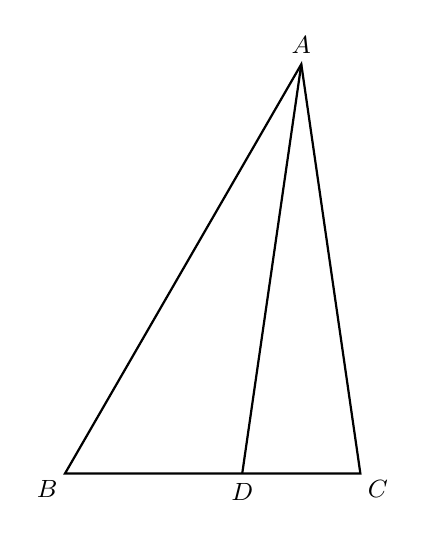
\begin{tikzpicture}[scale=0.75, line width=0.8pt, font=\small]
  \coordinate (B) at (0,0);
  \coordinate (D) at (3,0);
  \coordinate (C) at (5,0);
  \coordinate (A) at (4,6.9282);   % AB=8，∠B=60°

  \draw (A) -- (B) -- (C) -- cycle;
  \draw (A) -- (D);

  \node[above] at (A) {$A$};
  \node[below left=-1pt] at (B) {$B$};
  \node[below] at (D) {$D$};
  \node[below right=-1pt] at (C) {$C$};
\end{tikzpicture}
\end{center}
\nopagebreak[4]
（1） 求 $\sin\angle BAD$；

（2） 求 $BD$，$AC$ 的长。

\end{question}
\begin{question}
\gkti{16}李明在 $10$ 场篮球比赛中的投篮情况（假设各场比赛相互独立）：

\begin{center}
\begin{tabular}{llllll}
\toprule
场次 & 投篮次数 & 命中次数 & 场次 & 投篮次数 & 命中次数 \\
\midrule
主场 $1$ & $22$ & $12$ & 客场 $1$ & $18$ & $8$ \\
主场 $2$ & $15$ & $12$ & 客场 $2$ & $13$ & $12$ \\
主场 $3$ & $12$ & $8$ & 客场 $3$ & $21$ & $7$ \\
主场 $4$ & $23$ & $8$ & 客场 $4$ & $18$ & $15$ \\
主场 $5$ & $24$ & $20$ & 客场 $5$ & $25$ & $12$ \\
\bottomrule
\end{tabular}
\end{center}

（1） 从上述比赛随机选择一场，求李明在该场比赛中的投篮命中率超过 $0.6$ 的概率；

（2） 从上述比赛随机选择一个主场和客场，求李明的投篮命中率一场超过 $0.6$，一场不超过 $0.6$ 的概率；

（3） 记 $\bar x$ 是表中 $10$ 个命中次数的平均数，从上述比赛中随机选择一场，记 $X$ 为李明在这场比赛中命中次数，比较 $E(X)$ 与 $\bar x$ 的大小。（只需写出结论）

\Needspace{0.4\textheight}
\end{question}
\begin{question}
\gkti{17}如图，正方形 $AMDE$ 的边长为 $2$，$B$，$C$ 分别为 $AM$，$MD$ 的中点，在五棱锥 $P\text{-}ABCDE$ 中，$F$ 为棱 $PE$ 的中点，平面 $ABF$ 与棱 $PD$，$PC$ 分别交于点 $G$，$H$。
\nopagebreak[4]
\begin{center}% ============================================================
% f2014_beijing_science_q17_pyramid.tex
% 2014 北京卷（理科）第 17 题：五棱锥 P-ABCDE
% 来源 PDF：普通高考/2014/2014北京理.pdf
% 原页：第 1 页（A3），印面 861，右栏第 17 题题干下方
% 底面为正方形 AMDE（边长 2）截去 △MBC，B、C 分别为 AM、MD 中点；
% F 为 PE 中点，截面 ABF 与 PD、PC 交于 G、H，截面为五边形 ABHGF。
% 斜二测投影：px = X + 0.52Y，py = Z + 0.62Y（再乘 1.6 作尺寸）。
% ============================================================
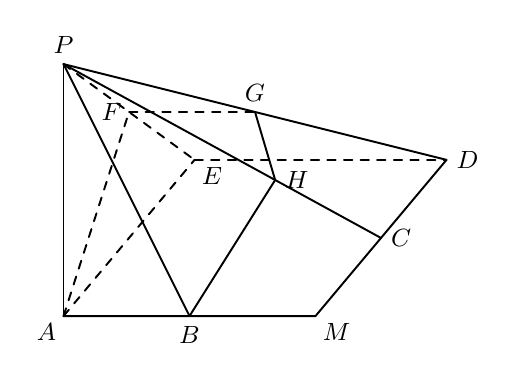
\begin{tikzpicture}[line width=0.7pt, font=\small,
  line cap=round, line join=round]
  % 顶点（斜二测投影后的纸面坐标）
  \coordinate (P)  at (0,3.200);
  \coordinate (A)  at (0,0);
  \coordinate (B)  at (1.600,0);
  \coordinate (M)  at (3.200,0);
  \coordinate (C)  at (4.032,0.992);
  \coordinate (D)  at (4.864,1.984);
  \coordinate (E)  at (1.664,1.984);
  \coordinate (F)  at (0.832,2.592);  % PE 中点
  \coordinate (G)  at (2.432,2.592);  % PD 中点
  \coordinate (H)  at (2.688,1.728);  % PC 上，PH:HC=2:1

  % 被遮挡的棱与截面边
  \draw[dashed] (P) -- (E);
  \draw[dashed] (A) -- (E);
  \draw[dashed] (E) -- (D);
  \draw[dashed] (A) -- (F);
  \draw[dashed] (F) -- (G);

  % 可见的棱
  \draw (P) -- (A);
  \draw (P) -- (B);
  \draw (P) -- (C);
  \draw (P) -- (D);
  \draw (A) -- (B) -- (M) -- (C) -- (D);

  % 可见的截面边
  \draw (B) -- (H) -- (G);

  % 标注
  \node[above] at (P) {$P$};
  \node[left=-1pt] at (F) {$F$};
  \node[above] at (G) {$G$};
  \node[right] at (H) {$H$};
  \node[below right=-1pt] at (E) {$E$};
  \node[below left=-1pt] at (A) {$A$};
  \node[below] at (B) {$B$};
  \node[below right=-1pt] at (M) {$M$};
  \node[right] at (C) {$C$};
  \node[right] at (D) {$D$};
\end{tikzpicture}
\end{center}
\nopagebreak[4]
（1） 求证：$AB\parallel FG$；

（2） 若 $PA\perp$ 平面 $ABCDE$，且 $PA=AE$，求直线 $BC$ 与平面 $ABF$ 所成角的大小，并求线段 $PH$ 的长。

\end{question}
\begin{question}
\gkti{18}已知函数 $f(x)=x\cos x-\sin x$，$x\in\left[0,\dfrac\pi2\right]$。

（1） 求证：$f(x)\leqslant 0$；

（2） 若 $a<\dfrac{\sin x}x<b$ 在 $\left(0,\dfrac\pi2\right)$ 上恒成立，求 $a$ 的最大值与 $b$ 的最小值。

\end{question}
\begin{question}
\gkti{19}已知椭圆 $C:x^2+2y^2=4$。

（1） 求椭圆 $C$ 的离心率；

（2） 设 $O$ 为坐标原点，若点 $A$ 在椭圆 $C$ 上，点 $B$ 在直线 $y=2$ 上，且 $OA\perp OB$，试判断直线 $AB$ 与圆 $x^2+y^2=2$ 的位置关系，并证明你的结论。

\end{question}
\begin{question}
\gkti{20}对于数对序列 $P:(a_1,b_1),(a_2,b_2),\cdots,(a_n,b_n)$，记 $T_1(P)=a_1+b_1$，$T_k(P)=b_k+\max\{T_{k-1}(P),a_1+a_2+\cdots+a_k\}$（$2\leqslant k\leqslant n$），其中 $\max\{T_{k-1}(P),a_1+a_2+\cdots+a_k\}$ 表示 $T_{k-1}(P)$ 和 $a_1+a_2+\cdots+a_k$ 两个数中最大的数。

（1） 对于数对序列 $P:(2,5),(4,1)$，求 $T_1(P)$，$T_2(P)$ 的值；

（2） 记 $m$ 为 $a$，$b$，$c$，$d$ 四个数中最小值，对于由两个数对 $(a,b)$，$(c,d)$ 组成的数对序列 $P:(a,b),(c,d)$ 和 $P':(c,d),(a,b)$，试分别对 $m=a$ 和 $m=d$ 时两种情况比较 $T_2(P)$ 和 $T_2(P')$ 的大小；

（3） 在由 $5$ 个数对 $(11,8)$，$(5,2)$，$(16,11)$，$(11,11)$，$(4,6)$ 组成的所有数对序列中，写出一个数对序列 $P$ 使 $T_5(P)$ 最小，并写出 $T_5(P)$ 的值。（只需写出结论）

\end{question}